% vim: spelllang=en spell textwidth=120
\documentclass[deska]{subfiles}
\begin{document}

\chapter{Server part of deska}
\label{sec:deska-server}

\begin{abstract}
Talk about server part of deska application. Deska server application and deska database.
\end{abstract}

\section{Server and its database}
Server part of deska application can be divided into two parts. The {\em deska-server} and {\em deska-database}.
Deska-server is python application, that runs for every user, listen for the commands from deska-cli (see DBAPI protocol).
Main work is to load json data, call corresponding stored function, and return the answer to deska-cli.
There are some special functions (freezeChangeset, showConfigDiff etc.) that are not implemented by deska db, but the server itselfs.

\section{Deska-server}
\todo{Lukas: about deska server configuration generators \& some tricks (maybe) in deska-server to explain.}

\section{Deska-database}
Deska-database is Postgresql database server, storing all data of user given schema, its relations and all changes of data.
There are tables, specified by user before build deska-database, tables for history tracking and many function for data manipulation.

\subsection{Data storage}
To prevent misunderstanding, if we talk about database, we use word {\em schema} in two different meanings. {\em User defined schema},
with meaning tables, with constraints describing data, that user wants to store into database. And {\em schema}, term used by
Postgresql with meaning something as namespace containing database objects (tables, types, functions etc).
It is similar to Oracle's package. If we talk about user defined schema, we write the whole term, and if we talk about schema, we write
schema plus its name.

Lets look at how data are stored in deska database. Three types of data are stored in deska-database.

At first, there are information
about user defined database schema. These information are provided by {\tt kindNames}, {\tt kindAttributes} and {\tt kindRelations} functions.
Although of many these information can be read from database catalog, there are stored in {\tt generated.py} file, which is used by
functions listed above, to get asked information. This kind of implementation, does not need access to database catalog or any table.

Second, the why we are here - the meaning of life, user data, fitting into user defined schema.
Objects and its attributes are stored in tables. 
After changeset is started, all data stored into database, are place into tables in history schema. Every kind has table in history
schema, with all attributes defined in user defined schema, and some more for history tracking.
There are tables defined by user, stored in schema production. These tables
(with its constraints) are used for validate data when committing changeset, if data are successfully copied into tables in schema production,
from tables in schema history data are valid, corresponding to user defined schema.
See \secref{sec:versioning} for more info.

Third, there has to be some information about revisions and changeset. There are two tables, version (the name was here before
we start using {\em revision}) and changeset, for storing information about revisions and changeset. These tables are
in versioning schema.

\subsection{Data manipulation}
For manipulation with stored data, there is many stored procedures, in Postgresql called {\em functions}.
Every action on data, as create object, set attribute, delete object, get object data, create changeset, delete changeset etc.,
has a function that do that. For object and its attributes, there are in genproc schema and are generated by
\todo{Martina: how we call generator this exactly?}
For changesets and versions, there are written by hand, and stored in deska schema, with many helping functions.

\subsection{Communication}
All communication with deska-server is implemented in schema json. There are functions, written in pg-python, which use another
functions, to manipulate with data in database. Or get data directly from tables as in {\tt pendingChangeset} and {\tt listRevisions}
\footnote{This direct access is not shown in the picture}.
Why we created this layer, and why it returns json data and not table or normal value, will be described in section Json schema.
See \secref{sec:schema-json} for more info.

The picture shows how deska-server and deska-database communicate. Schema json provides interface for deska-server. It
calls functions from other schemas (genproc and deska). All these schemas are drawn as components. Schemas containing
tables are shown in different form, because they do not provide real interface.
\begin{figure}[h]
	\centering
	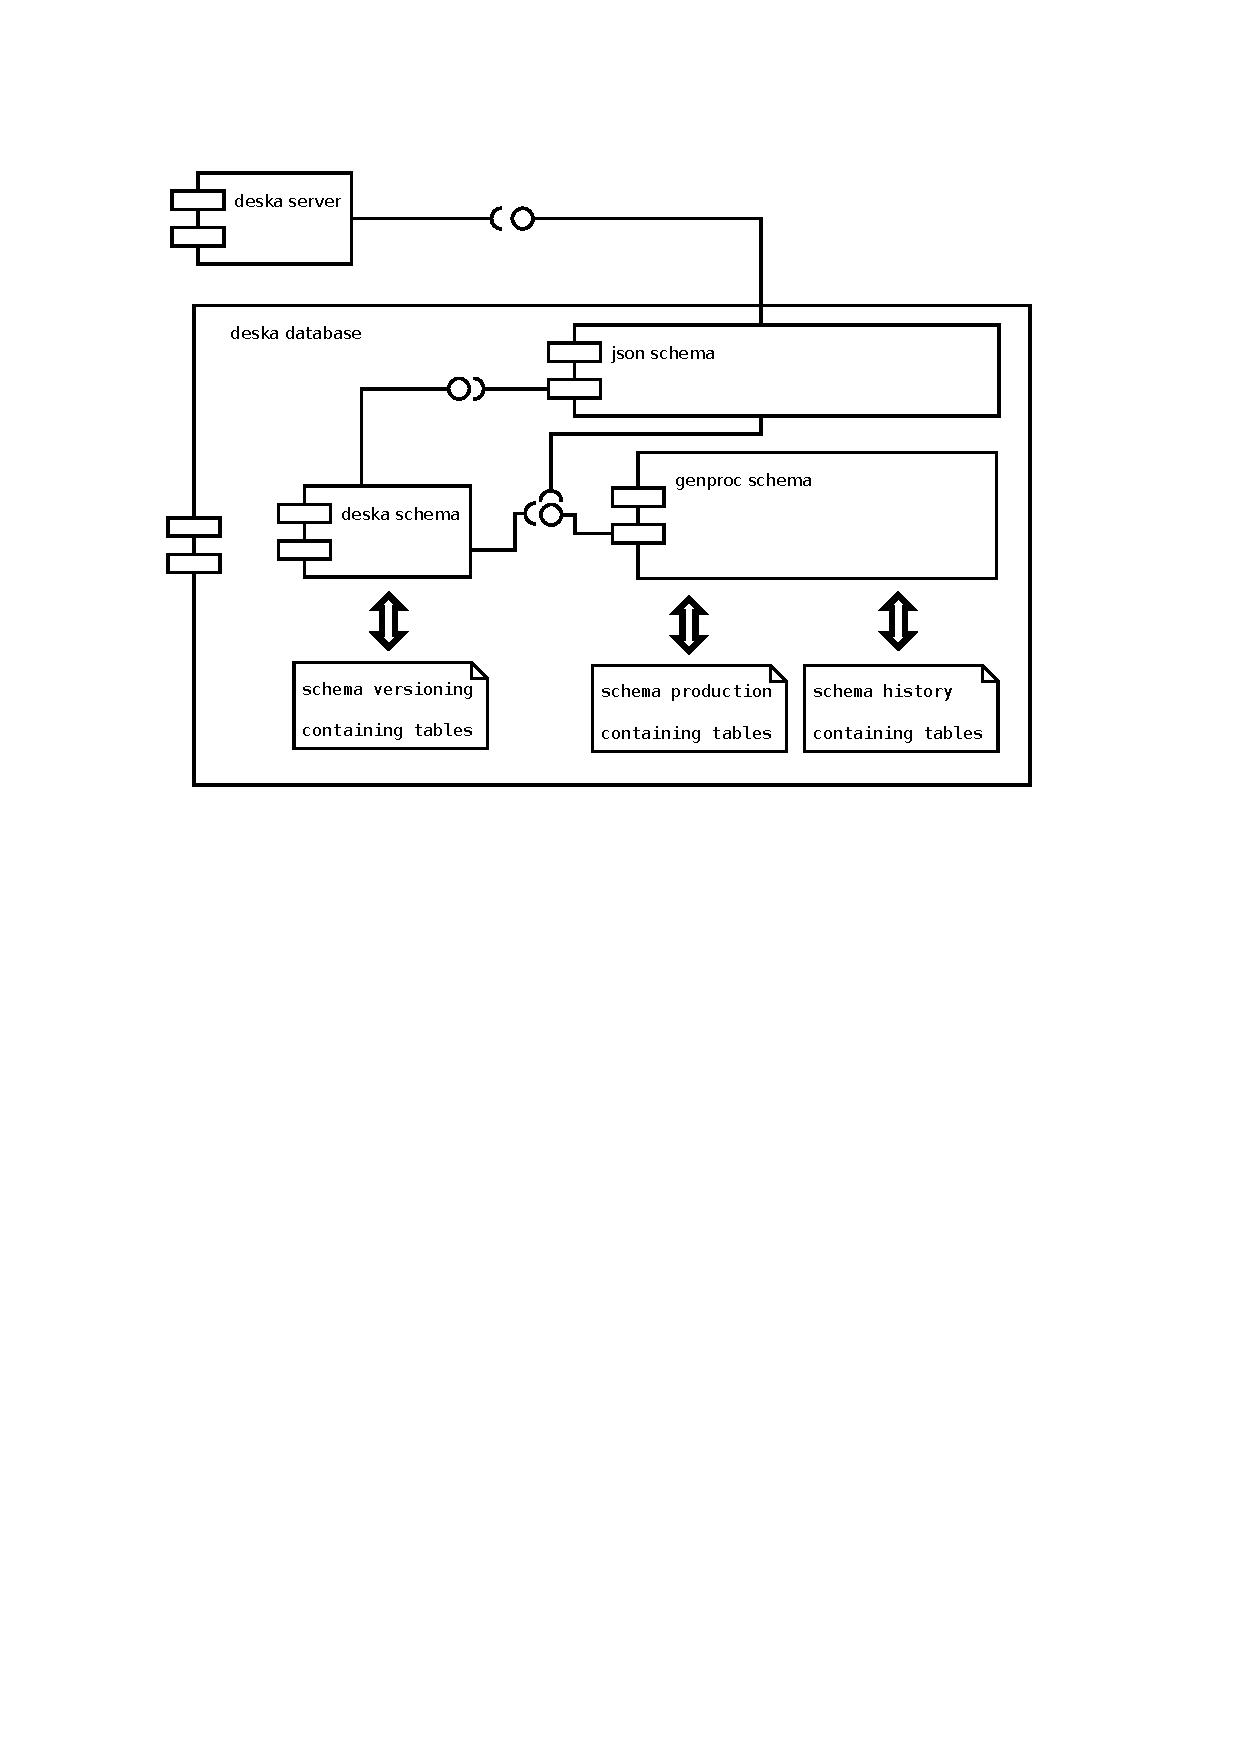
\includegraphics[trim=28mm 170mm 30mm 28mm]{img-deska-server-components.pdf}
	\caption{Deska server components}
\end{figure}

\subsection{Json schema}
\label{sec:schema-json}
After we have generated functions for manipulating with data, and DBAPI specified, it was clear, that there must be some layer,
that transforms createObject(kindName,xxx) to kindName\_add(xxx), which is call of generated SQL function.
We do that in deska-database, because we wanted to have 1:1 mapping between database functions, and DBAPI commands.

It works well until first performance testing was made. The state was, that deska-server call for data - millions of objects,
database worked and worked and... when finally returned this data to server, server started transformation... It takes long time
and consumes lots of memory.
In the same time, diffing implementation started, and there where problems with many functions of different result types,
that has to be called, which was hard to union into one function.
So there was an idea, that json can be created inside database, so that the union of diffing function can return json.

Some test were run, the time for smaller data was worse with json in database, but for large data, there was significant
speed up. The function written in pg-python creates part of the json structure in each line of database cursor.
So the json structure grows up with data that database produced.
\todo{Lukas: get results of these tests}

The result is, that every function callable by server returns json.

\subsection{Getting data from tables}
\label{sec:data-functions}
Here we talk about getting data of objects, revisions and changesets stored in tables.
There are {\tt pendingChangeset} that selects data from changeset table, and {\tt listRevisions} that selects data from version table.
Both accept filter as parameter and uses some cast optimization, about which we will talk in section about cast
optimization \secref{sec:cast}.

Object data functions {\tt objectData}. {\tt resolvedObjectData}. {\tt resolvedObjectDataWithOrigin} calls generated functions 
that returns tuple of attribute values, that is just converted into json format and returned. 

Functions {\tt multipleObjectData}. {\tt multipleResolvedObjectData} and {\tt multipleResolvedObjectDataWithOrigin} has parameter revision.
Postgresql does not have parametrized view, so we have to use function, to implement it. How this fact complicates filtering will
be described in section \secref{sec:filter-speed}

In this function, more work is done, than in another json schema function, that only runs some function.
There is still only one main call another database function (and one helping, to get revision number).
But the SQL statement to run is created in more difficult way. In contrast to other json functions,
here we creates complicated column definition for the SQL statement. It goes between SELECT and FROM keywords.

It contains definition of all columns that shall be returned in human readable form.
In database tables, reference columns has bigint type, but user wants to see text name of referenced kind.
The sets are represented by another table, but user wants to see array etc. So some transformation must be done.
Easiest it is for simple attribute,
for example if kind host has attribute note, than the column definition is {\em host.note}.
It gets complicated, when the attribute is part of some relation. For example refers\_to.
If host has attribute hardware, referencing to kind hardware. Than column definition is 
{\em hardware\_get\_name(host.hardware,\$1)}. For sets, templates and embed kinds it is similar.

\subsection{Getting data from tables - casting}
\label{sec:cast}
For performance reasons, in column definition, we do one more thing. It is casting.
In pg python extension, there is some function that from Postgresql types create native python types.
It is called Postgres.convert\_postgres\_objects
and must be called for every result from database. But it supports only some types.
And from these some types, some converts in different way than we want.

At first, we solve this with our own function, that do the transformation, but if it runs for every
row and every column, it was very slow. So we do most of this transformation using Postgresql cast
in SQL statements. It is much faster.
\todo{Lukas: some test results}

The column definition, is more complicated than we describe above. If
Postgres.convert\_postgres\_objects function 
does not support conversion, or do in bad way for us, we add cast in column definition.
For example if there is timestamp attribute, we add {\em ::text}, if it is ipv4 type, and we don't want
the conversion with mask suffix, we use {\em host} function in column definition.


\subsection{Filters}

Some functions (lets call them {\em data functions} in json schema have parameter filter. It is in json format,
see DBAPI protocol in~\secref{sec:api-filters} for more info.
The data function, in json schema, have part where SQL statement is created. It is described in
\secref{sec:data-functions}.

This filter is implemented in filter.py file in class Filter.
It add JOIN and WHERE parts to the SQL statement that is used by data functions. So that Filter class has
methods getJoin and getWhere that returns strings which fits at the end of SQL statement in data function.

Filter constructor parses given filter into parts - conditions.
Every condition has kind, attribute, operator and value. From this we create strings line
{\em kind.attribute = kind2\_get\_uid(\$2)}. If there is more conditions, they are joined with AND or OR
operators.
If kind in condition is different from kindName - function parameter, it is remember,
and in getJoin function, if it is possible, string like {\em JOIN kind2 ON kind2.uid = kind.attribute}
is returned. This is possible when some relation between this kinds exists.
If there is more different kinds, join string with more JOINs is produced.
Information about relation are taken from generated.py file.

It was add into deska later than other functions, so that it uses what was developed before.

\subsection{Filters limitations}
\label{sec:filter-speed}
As we say, filtering requirement was add very late. In that time, data functions has parameter revision
and only way to implement this is via function returning table.

So the filter is applied on the result of this function, providing parametrized view.
It is hard to say, if firstly you have to select data in some revision and than apply filter,
or firstly apply filter and then select revision of this data. It depends on concrete query.

But main problem is not, what to select at first. It is that table returning function has
no indexes and every filtering is done by full table scan.
This slows filters down, and it must be improved in the future. It is not hard,
if you use view instead of function simulating parametrized view, indexes can be used.
And as we can see, revision parameter is not used now, so if DBAPI specification changes,
we can transform this functions into views. Or someone can also do view and function
and use view in no parameter revision is specified.

\subsection{Error handling}
Here we try to explain work with exceptions in deska-database and deska-server. Postgresql functions can RAISE exception with given message and sqlstate.
This sqlstate is like number of error. We use this to split possible exceptions into some category - exception types. Exception in database is
every unexpected or “bad” thing that occurs. It can be run time error as well as constraint violation, or exception thrown explicitly by RAISE.

While json schema provide json as returned types, we try to catch maximum number of exception inside the database (in
json schema part).
For this catching DeskaException class is used. It has constructor, with Postgresql.dberr as parameter, which is structure that contains exception
message, and sqlstate. We use this information to determine exception type - class contains typeDict - dictionary {sqlstate: exceptionType}.
Finally this function has json method, which takes name on the function, in which error occurs and creates exception in json format.

\todo{Lukas: exceptions on server}

\end{document}
